% Appendix Template

\chapter{Instrucciones} % Main appendix title

\label{App_Inst} % Change X to a consecutive letter; for referencing this appendix elsewhere, use \ref{AppendixX}

En el presente apéndice se incluye una copia exacta de las instrucciones e indicaciones que fueron leídas al inicio de cada uno de los Subjuegos 1 y 2 que conformaron las 10 distintas sesiones experimentales realizadas.\\

\section{Instrucciones para todos los participantes al inicio de la sesión}

Hola a todos y gracias por venir. Este es un experimento sobre toma de decisiones y no queremos que influyan sobre las decisiones de los demás. Por lo tanto, no está permitido que hablen o se comuniquen entre ustedes.\\

Si tienen alguna duda levanten la mano e iré a su lugar para resolverla.\\

En este experimento, van a participar en un juego que se repite cuatro veces. Llamaremos a cada repetición del juego un \underline{Periodo}. En el juego sólo participan tres personas. Mediante un sorteo, elegiremos a tres de ustedes para que jueguen primero, mientras los otros dos esperarán en otra aula. Cuando las primeras tres personas terminen de jugar por cuatro periodos, se elegirá a una de estas tres personas para que juegue junto con las dos personas que estaban esperando. Cuando este segundo grupo termine de jugar cuatro veces, terminará el experimento.\\

En cada periodo podrán ganar puntos de juego. Por el hecho de participar en este experimento, todos tienen medio punto sobre su examen parcial, y al final de los cuatro periodos, el participante que haya acumulado más puntos de juego ganará otro medio punto sobre su examen parcial, por lo que pueden ganar hasta un punto completo sobre su examen. En caso de empates, el medio punto se dividirá entre los ganadores. En cada periodo, un jugador puede ganar hasta 8 puntos de juego, pero esto dependerá del desempeño de todos los participantes.\\

\begin{center}
\textit{[Entregar cuatro (\textit{4}) formatos de respuesta a cada participante. Cada participante debe recibir formatos con los números del 1 al 4 y con su clave personal.]}\\
\end{center}

Le estoy entregando cuatro formatos de respuesta a cada uno. Noten que los formatos que cada uno recibió tienen una combinación de números y letras en la celda llamada \underline{Clave}. Esta clave es única para cada uno de ustedes y la usaremos para identificarlos.\\

Los formatos también contienen una celda llamada \underline{Periodo} que contiene un número del 1 al 4. En cada periodo de juego, usarán únicamente el formato de respuesta que corresponda al periodo que se está jugando, es decir, el formato que dice Periodo 1 en el primer juego, el formato que dice Periodo 2 en el segundo juego, y así sucesivamente.\\

¿Cómo se juega? En cada periodo, cada jugador debe elegir un número entero entre el $0$ y el $100$. Deberán escribir su número en el formato de respuesta, en la celda llamada \underline{Mi Número Elegido}. No dejen que los otros participantes conozcan el número que eligieron.\\

El ganador de ese periodo será el participante cuyo número elegido esté lo más cercano posible al \underline{Número Objetivo} de ese periodo. ¿Cuál es el Número Objetivo? El Número Objetivo se calcula de la siguiente manera:\\

Se obtiene el promedio de los números elegidos por cada jugador, es decir, se suman los tres números y se divide entre 3. Después, este número promedio se multiplica por $frac{2}{3}$, es decir se multiplica por 2 y se divide entre 3. El resultado es el Número Objetivo.\\

En otras palabras, para ganar deberán elegir un número que crean que estará lo más cerca posible al promedio de los números elegidos por todos los participantes, multiplicado por $frac{2}{3}$,. El ganador obtendrá 6 puntos de juego. Si dos o los tres de ustedes eligen números igual de cercanos al Número Objetivo, los 6 puntos de juego se dividirán equitativamente entre todos los participantes ganadores.\\

Como verán, hay una celda más en su formato de respuesta, llamada \underline{Números de los otros Jugadores} que contiene espacio para que escriban dos números. Lo que deben hacer en cada periodo después de elegir su propio número es escribir en esta celda dos números enteros que ustedes crean que estarán lo más cerca posible a los números que van a elegir los otros dos participantes. En otras palabras, deben intentar adivinar qué números elegirán los otros jugadores.\\

Ganarán 1 punto de juego si uno de los otros participantes elige para el juego un número hasta 5 números por arriba o por debajo de uno de los números que escribieron en la celda de Números de los otros Jugadores. Ganarán otro punto de juego si el otro participante elige un número hasta 5 números por arriba o por debajo de su segundo número escrito en la celda de Números de los otros Jugadores.
Es decir, sólo ganarán dos puntos si sus dos números se acercan a los dos números de los otros jugadores.\\

\begin{center}
\textit{[Escribir en el pizarrón: $X \frac{+}{-}5$ y $Y \frac{+}{-}5$]}\\
\end{center}

Ustedes eligen dos \underline{Números de los otros Jugadores}, $X$ y $Y$. Si ambos jugadores eligen un número que está dentro del rango de $X \frac{+}{-}5$, pero ninguno de los dos entra en el rango de $Y \frac{+}{-}5$, entonces sólo ganarán un punto. Para que sea posible ganar el segundo punto, el número de uno de los otros jugadores debe caer dentro de $X \frac{+}{-}5$ y el otro dentro del rango de $Y\frac{+}{-}5$. Si creen que los otros jugadores van a elegir números muy cercanos, es válido elegir números muy cercanos o incluso iguales.\\

Recuerden, los números que elijan para la celda Números de los otros Jugadores NO influyen en el valor del Número Objetivo ni influyen en determinar qué jugador gana en cualquier periodo. Los números de esta celda únicamente sirven para ganar puntos ADICIONALES si adivinan los números que los otros participantes escribieron en la celda Mi Número Elegido.\\

Una vez que hayan llenado todas las celdas del formato de respuesta para el periodo actual, coloquen su formato boca abajo y esperen a que los otros participantes terminen y hagan lo mismo. Una vez que todos hayan terminado, pasaré a sus lugares a recoger sus formatos de respuesta para este periodo. Escribiré en el pizarrón los tres números elegidos sin indicar a quién corresponde cada número, y usaré los números elegidos para calcular el promedio, que escribiré en el pizarrón. Multiplicaré el promedio por $\frac{2}{3}$  y escribiré este número, que será el Número Objetivo, en el pizarrón.\\

Revisaré cuál de los tres números elegidos es el más cercano al Número Objetivo, y si los números que escribieron en la celda Números de los otros Jugadores acertaron a los números elegidos por sus oponentes. En función a esto registraré cuántos puntos obtuvo cada quien en este periodo y se los haré saber de forma individual.\\

Borraré los números escritos en el pizarrón y comenzaremos el siguiente periodo, repitiendo el proceso.\\

\begin{center}
\textit{[Las personas con las claves A, B, y C juegan primero]}.\\
\end{center}

\section{Instrucciones para los participantes del subjuego 2}

Les repito brevemente las instrucciones. Van a repetir un juego cuatro veces. En cada repetición, o periodo, van a elegir un número entero entre $0$ y $100$ que escribirán en la celda \underline{Mi Número Elegido}. Ganará 6 puntos de juego el participante que haya elegido el número más cercano al promedio de los números elegidos por los todos participantes, multiplicado por $frac{2}{3}$.\\

En la celda \underline{Números de los otros Jugadores} deben escribir dos números enteros que crean que estarán lo más cerca posible de los números elegidos por los otros participantes. Ganaran 1 punto de juego por cada número que hayan escrito en esta celda que esté 5 números por arriba o por debajo de un número elegido por los otros jugadores.\\

Recuerden que uno de ustedes ya ha jugado este juego, mientras que dos de ustedes nunca lo han jugado.\\
 
\section{Formato de Respuesta}

Finalmente, se anexa un ejemplo del Formato de Respuesta empleado durante el experimento:

\begin{figure}[th]
\centering
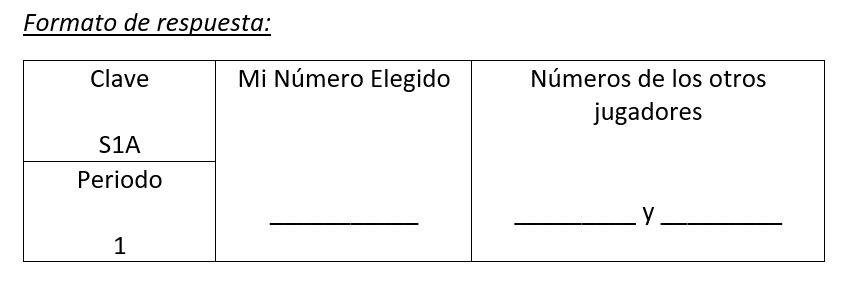
\includegraphics[width=0.90\textwidth]{Figures/FormatoRespuesta} 
%\decoRule
\caption[Formato de Respuesta muestra empleado en el experimento]{Formato de Respuesta estándar proporcionado a los participantes por cada uno de los cuatro periodos incluidos en cada subjuego}
\label{fig:DiferenciasNormalizadas_Subjuego1}
\end{figure}
